% Gemini theme
% See: https://rev.cs.uchicago.edu/k4rtik/gemini-uccs
% A fork of https://github.com/anishathalye/gemini

\documentclass[final]{beamer}

% ====================
% Packages
% ====================

\usepackage[T1]{fontenc}
\usepackage{lmodern}
\usepackage[size=custom,width=120,height=72,scale=1.0]{beamerposter}
\usetheme{gemini}
% \usecolortheme{uchicago}
\usecolortheme{stanford}
\usepackage{graphicx}
\usepackage{booktabs}
\usepackage{tikz}
\usepackage{pgfplots}
\pgfplotsset{compat=1.17}

% ====================
% Lengths
% ====================

% If you have N columns, choose \sepwidth and \colwidth such that
% (N+1)*\sepwidth + N*\colwidth = \paperwidth
\newlength{\sepwidth}
\newlength{\colwidth}
\setlength{\sepwidth}{0.025\paperwidth}
\setlength{\colwidth}{0.3\paperwidth}

\newcommand{\separatorcolumn}{\begin{column}{\sepwidth}\end{column}}


\title{An exploration on Wasserstein GAN and Pearson $\chi^2$ f-GAN}


\author{Enzo Jia \inst{1}}

\institute[shortinst]{\inst{1} Department of Computer Science}
\institute[shortinst]{\inst{1} Department of Computer Science, Stanford University}

% ====================
% Footer (optional)
% ====================

\footercontent{
  \href{https://github.com/enzochia/minBERT_CS224N}{https://github.com/enzochia/} \hfill
  % NeurIPS 2021 Workshop: Metacognition in the Age of AI \hfill
  \href{mailto:enzo.jia@gmail.com}{enzojia@stanford.edu [frequently-checked email: enzo.jia@gmail.com]}}
% (can be left out to remove footer)

% ====================
% Logo (optional)
% ====================

% use this to include logos on the left and/or right side of the header:
% \logoright{\includegraphics[height=7cm]{logos/cs-logo-maroon.png}}
% \logoleft{\includegraphics[height=7cm]{logos/cs-logo-maroon.png}}

% ====================
% Body
% ====================

\begin{document}

% This adds the Logos on the top left and top right
\addtobeamertemplate{headline}{}
{
    \begin{tikzpicture}[remember picture,overlay]
    %   \node [anchor=north west, inner sep=3cm] at ([xshift=0.0cm,yshift=1.0cm]current page.north west)
    %   {\includegraphics[height=5.0cm]{stanford_logos/Stanford-CS.png}}; % uc-logo-white.eps
      \node [anchor=north east, inner sep=3cm] at ([xshift=0.0cm,yshift=2.5cm]current page.north east)
      {
\includegraphics[height=7.0cm]{stanford_logos/Block_S_2_color.png}};
    \end{tikzpicture}
}

\begin{frame}[t]
\begin{columns}[t]
\separatorcolumn

\begin{column}{\colwidth}

  \begin{block}{Abstract: a problem statement}
   Generative Adversarial Nets (GAN) provides a straightforward yet effective method for image generation after learning from training data, and researchers have proposed variants under GAN framework. In this project I compare performances between Vanilla GAN, Wasserstein GAN (WGAN) and $f$-GAN, as the later two extend and generalize GAN implementations. Experimental results show that compared to vanilla GAN, WGAN and Pearson $\chi^2$ $f$-GAN have similar capacities on learning data distributions and generating, given features extracted by convolutional networks. This project also explores hyper parameter tuning for WGAN and the results emphasize importance of gradient clipping threshold.

  \end{block}

  \begin{block}{Introduction and optimization goals}
  
\begin{alertblock}{Vanilla GAN}
% {\bf Vanilla GAN} 
Goal of training a GAN is to have D (discriminator) to maximize the probability of correctly labeling an input image whether it is from actual data or generated by G (generator), and meanwhile to have G to minimize the probability that D labels generated images correctly. Thus we have loss:
\begin{equation} 
\begin{split}
\begin{aligned}
\underset{G}{\text{min}}\; \underset{D}{\text{max}}\; \mathbb{E}_{x \sim p_\text{data}}\left[\log D(x)\right] + \mathbb{E}_{z \sim p(z)}\left[\log \left(1-D(G(z))\right)\right]
\end{aligned}
\end{split}
\label{loss_gan}
\end{equation}
\end{alertblock}
\begin{alertblock}{Wasserstein-GAN (WGAN)}
% {\bf WGAN} 
For vanilla GAN the final output of its discriminator is modeled to be the probability of the input image being an actual image sampled from data and not generated. However there are other approaches we can consider, and one of them is Wasserstein-GAN (WGAN), which does not train its critic (discriminator) as an classifier outputting probabilities, but only trains it to give scores without the constraint of being between 0 and 1 \cite{arjovsky2017wasserstein}. WGAN optimizes the model by minimizing the Earth-Mover distance between model distribution and real data distribution.
\begin{equation} 
\begin{split}
\begin{aligned}
W(\mathbb{P}_r, \mathbb{P}_g) = \underset{\gamma \in \Pi(\mathbb{P}_r, \mathbb{P}_g)}{\text{inf}} \mathbb{E}_{(x, y) \sim\gamma}[||x - y||]
\end{aligned}
\end{split}
\label{em_i}
\end{equation}
\end{alertblock}
\begin{alertblock}{$f$-GAN}
% {\bf $f$-GAN} 
One perspective to see vanilla GAN's training procedure of the generator is minimizing a variant of the Jensen-Shannon divergence between the model distribution and real data distribution \cite{goodfellow2014generative}. Meanwhile we can generalize the Jensen-Shannon divergence to $f$-divergence family, also known as Ali-Silvey distances \cite{nowozin2016fgan}. Under this frame we have the loss function:
\begin{equation} 
\begin{split}
\begin{aligned}
    \underset{\theta}{\text{min}}\; \underset{w}{\text{max}} \; \mathbb{E}_{x\sim P} [g_f(V_w(x))] + \mathbb{E}_{x\sim Q_\theta} [-f^*(g_f(V_w(x)))]
\end{aligned}
\end{split}
\label{f_divergence_obj_ii}
\end{equation}
\end{alertblock}
  \end{block}
\begin{block}{Experiment settings}
{\bf Design}. This project explores into 3 dimensions, and the goal is to find an optimized combination of approaches on high level framework and low level modeling. 
\begin{itemize}
    \item {\bf Framework}. Performance difference between 3 GAN variants as discussed above.
    \item {\bf Model}. Performance difference of GANs with vs. without Conv layers in their model networks.
    \item {\bf Model}. Hyper parameter tuning for WGAN. 
\end{itemize}

{\bf Data}. This project uses the training set of MNIST data, from which I randomly select 50000 images for model training and 5000 for model validation. 

{\bf Metrics}. Tables of generated images are plotted for comparison. 


\end{block}





\end{column}

\separatorcolumn

\begin{column}{\colwidth}
  
    \begin{block}{Algorithms for GAN, WGAN, and $f$-GAN}
According to different optimization goals discussed in previous section, I derive Algorithm 1, with lines in black font are shared by all 3 GAN variants, and green lines only for Vanilla GAN, blues lines only for WGAN, and red lines only for Pearson $\chi^2$ $f$-GAN. 

\begin{table}[t]
  \centering
  \begin{tabular}{lcr}
   {\bf Algorithm 1} GAN, WGAN, and $f$-GAN. k is number of steps to apply to the discriminator. \\
   In the original papers {\color{green} [Vanilla GAN] k = 1.}  {\color{blue} [WGAN] k = 5.}  {\color{red} [$f$-GAN] k = 1.}\\ \hline
   {\bf for} number of training iterations {\bf do}\\
   \hspace{4mm} {\bf for} k steps {\bf do}\\
   \hspace{8mm} Sample minibatch of $m$ noise samples ${z^{(1)}, ..., z^{(m)}}$ from noise prior $p_g(z)$\\
   % $p_g(z)$\\
   \hspace{8mm} Sample minibatch of $m$ image samples ${x^{(1)}, ..., x^{(m)}}$ from data generating distribution $\mathbb{P}_r(x)$\\
   \hspace{8mm} {\color{red} [$f$-GAN] Apply $g_f$ as final layer activation function. For Pearson $\chi^2$ it is identical function.} \\   
   \hspace{8mm} Update the discriminator with chosen optimizer using gradient: \\
   \hspace{16mm} {\color{green} [Vanilla GAN] $\nabla_{\theta_d} \frac{1}{m} \Sigma_{i=1}^m [\log D(x^{(i)}) + \log (1 - D(G(z^{(i)})))]$} \\
   \hspace{16mm} {\color{blue}[WGAN] $\nabla_{w} [\frac{1}{m} \Sigma_{i=1}^m f_w(x^{(i)}) + \frac{1}{m} \Sigma_{i=1}^m  f_w(g_\theta(z^{(i)}))]$} \\
   \hspace{16mm} {\color{blue} [WGAN] w $\xleftarrow{}$ clip(w, -c, c)}\\
   \hspace{16mm} {\color{red} [$f$-GAN] $\nabla_{w} [\frac{1}{m} \Sigma_{i=1}^m g_f(V_w(x^{(i)})) - \frac{1}{m} \Sigma_{i=1}^m f^*(g_f(V_w(z^{(i)})))]$, which for Pearson $\Chi^2$ is:}\\
   \hspace{16mm} {\color{red} [$f$-GAN] $\nabla_{w} [\frac{1}{m} \Sigma_{i=1}^m V_w(x^{(i)}) + \frac{1}{m} \Sigma_{i=1}^m \left( \frac{1}{4} V_w(z^{(i)})^2 + V_w(z^{(i)})\right)]$}\\


   
   \hspace{4mm} {\bf end for} \\
   \hspace{4mm} Sample minibatch of $m$ noise samples ${z^{(1)}, ..., z^{(m)}}$ from noise prior $p_g(z)$\\
   \hspace{4mm} Update the discriminator with chosen optimizer using gradient: \\
   \hspace{16mm}  {\color{green} [Vanilla GAN]$\nabla_{\theta_g} \frac{1}{m} \Sigma_{i=1}^m \log (1 - D(G(z^{(i)})))$} \\   
   \hspace{16mm} {\color{blue} [WGAN] $\nabla_{\theta} \frac{1}{m} \Sigma_{i=1}^m f_w(g_\theta(z^{(i)}))$ }\\   
   \hspace{16mm} [$f$-GAN] {\color{red} $\nabla_{w} [\frac{1}{m} \Sigma_{i=1}^m f^*(g_f(V_w(z^{(i)})))]$, which for Pearson $\Chi^2$ is:}\\
   \hspace{16mm} [$f$-GAN] {\color{red} $\nabla_{w} [ - \frac{1}{m} \Sigma_{i=1}^m \left( \frac{1}{4} V_w(z^{(i)})^2 + V_w(z^{(i)})\right)]$}\\
   
   {\bf end for} \\ \hline
  \end{tabular}
  \label{algo_gan}
\end{table}

    \end{block}



\begin{block}{Eexpriment results: GAN variants and Conv layers}

\begin{figure}
\centering
\begin{tabular}{ccc}
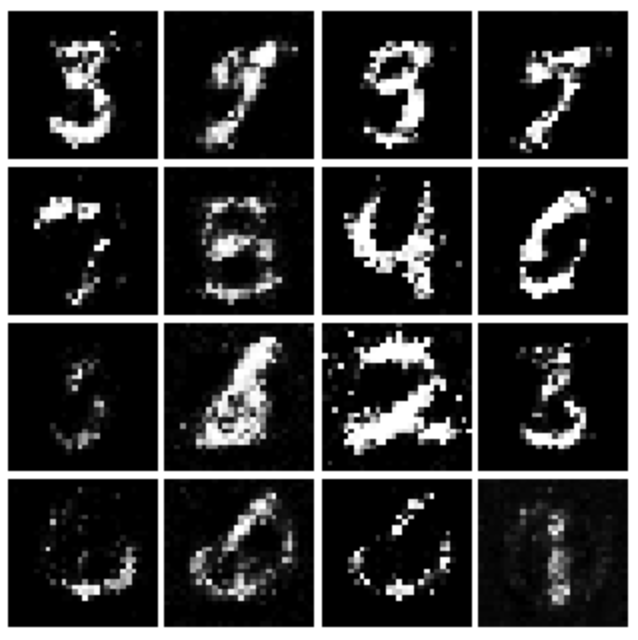
\includegraphics[width=100mm]{GAN_poster/GAN_noConv.png} & 
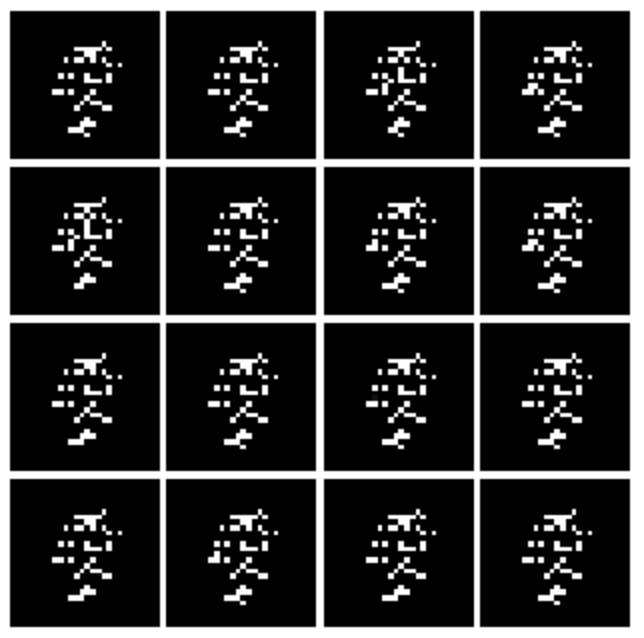
\includegraphics[width=100mm]{GAN_poster/WGAN_noConv.png} & 
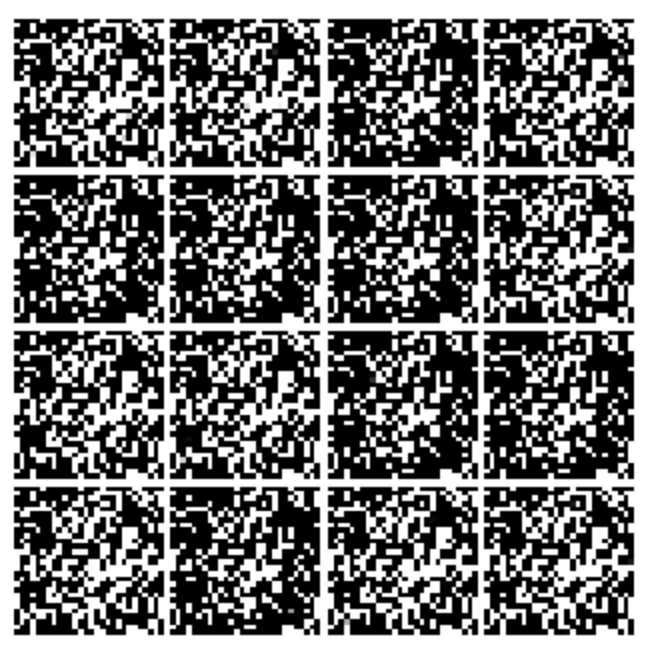
\includegraphics[width=100mm]{GAN_poster/fGAN_noConv.png} \\
(a)GAN, no Conv  & (b) WGAN, no Conv  & (c)$f$-GAN, no Conv  \\
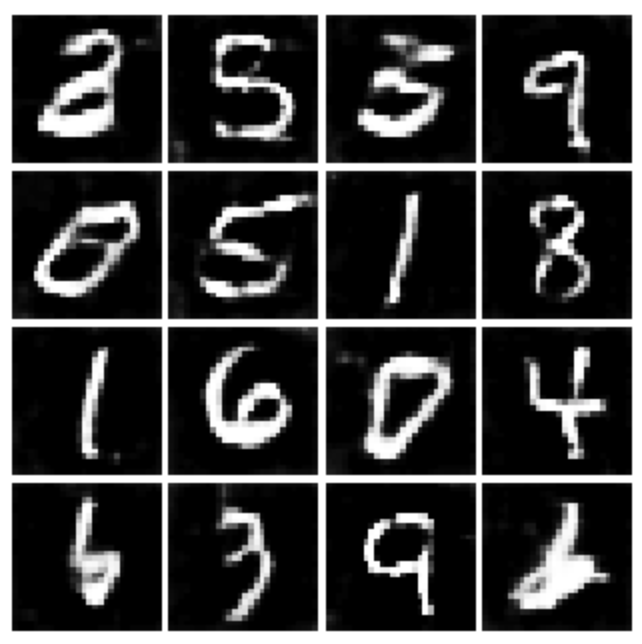
\includegraphics[width=100mm]{GAN_poster/GAN_Conv.png} & 
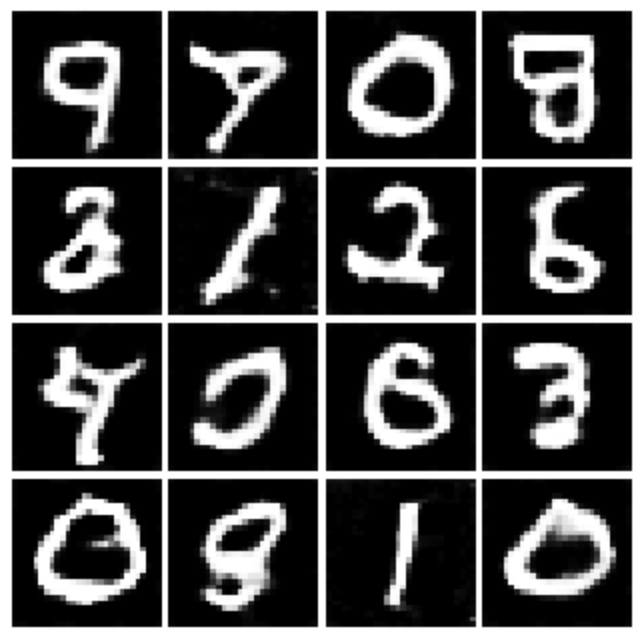
\includegraphics[width=100mm]{GAN_poster/WGAN_Conv.png} & 
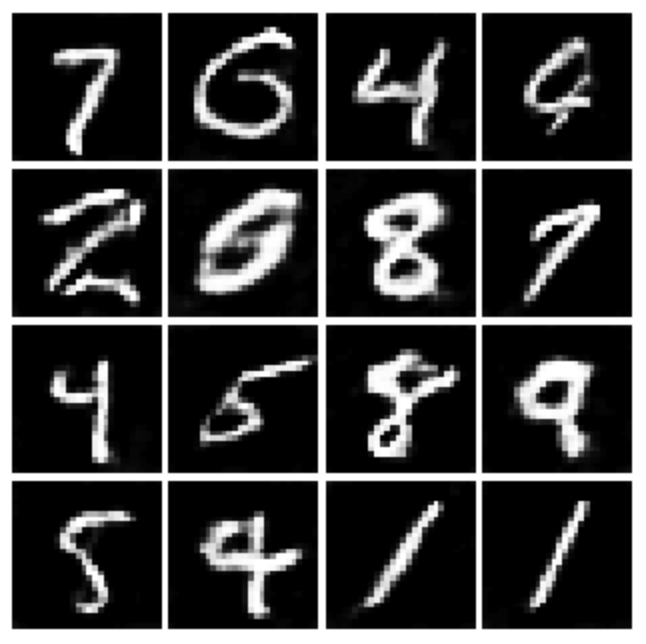
\includegraphics[width=100mm]{GAN_poster/fGAN_Conv.png} \\
(a)GAN, with Conv  & (b) WGAN, with Conv  & (c)$f$-GAN, with Conv  \\[6pt]
\end{tabular}
\caption{Digit images generated by Vanilla GAN, WGAN, and $f$-GAN, with and without Convolution layers for feature extractions, respectively.}
\label{gans_conv}
\end{figure}



\end{block}


% \begin{block}{Topics left for future work}
% \begin{itemize}
%     \item Loss function exploration for sentiment analysis. Cross entropy loss sees model outputs as categorical classfication results, however for sentiment analysis the label is ordinal data, with information unused.
%     \item More training data, including CFIMDB data for sentiment analysis.
%     \item Different foundation models.
%     \item Different experiment settings, including different optimizers, learning rates, etc.
% \end{itemize}
% \end{block}

\end{column}

\separatorcolumn

\begin{column}{\colwidth}


  \begin{block}{Experiment results: gradient clipping for WGAN}

\begin{figure}
\centering
\begin{tabular}{ccc}
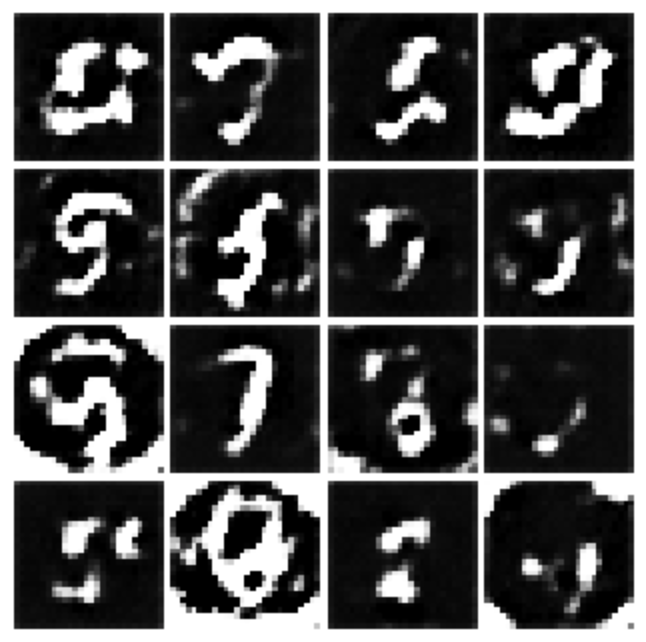
\includegraphics[width=100mm]{GAN_poster/WGAN_1e_n5_p001.png} & 
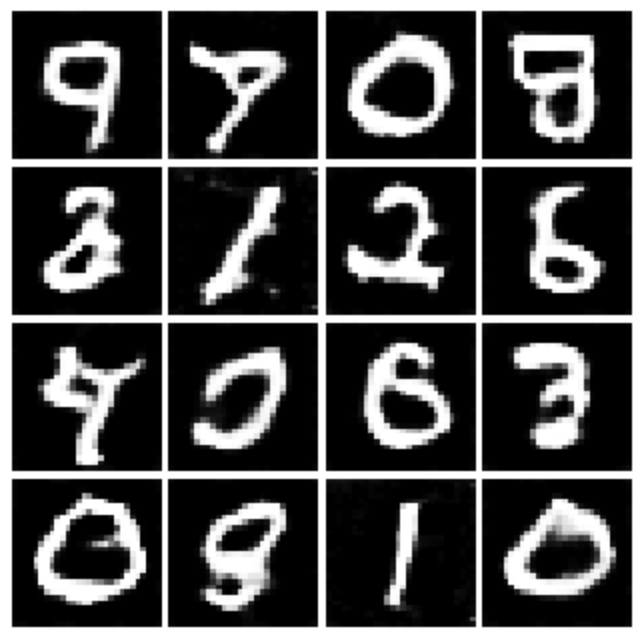
\includegraphics[width=100mm]{GAN_poster/WGAN_7p5e_n8_p001.png} & 
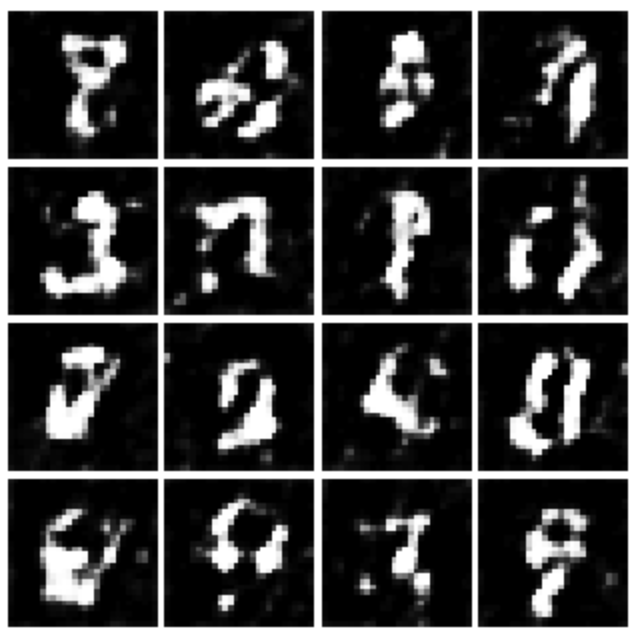
\includegraphics[width=100mm]{GAN_poster/WGAN_1e_n10_p001.png} \\
(a)gradient clipped at $1e-5$  & (b) gradient clipped at $7.5e-8$  & (c)gradient clipped at $1e-10$  \\[6pt]
\end{tabular}
\caption{Digit images generated by WGAN, with different gradient clipping thresholds. All 3 has weight clipped at 0.001.}
\label{WGAN_gradient_clip}
\end{figure}

  
  \end{block}



  \begin{block}{Discussions}
\begin{itemize}
    \item {\bf Vanilla GAN vs. WGAN vs. $f$-GAN} using features extracted by convolutional networks generate digit images of similar qualities, and meanwhile Pearson $\chi^2$ $f$-GAN generates with arguably better quality because its handwriting style aligns better with human handwriting habits. Most generated digits are readable, with small numbers of them being distorted. These three GAN variants' generations have recognizable different styles, for example WGAN's digit images have thicker strokes.
    \item {\bf Fully connected layers vs. convolutional networks}. Convolutional networks extract higher-quality image features, as for each GAN variant it performs better using convolutional networks.
    \item {\bf WGAN tuning}. When gradient clipping threshold is too small ($1e-10$) it has a high probability to cause vanishing gradient thus more random noisy images, and too large clipping threshold ($1e-5$) makes the network unstable and thus generates more distorted digits.   
    \item {\bf WGAN tuning}. On weight clipping threshold dimension, we have similar observation as gradient clipping threshold. Not included in figure \ref{WGAN_gradient_clip}. 

\end{itemize}  



  \end{block}

  \begin{block}{Conclusions}
In this project I implement Vanilla GAN, WGAN and Pearson $\chi^2$ $f$-GAN, with and without convolutional layers. The results prove that under help of features extracted by convolutional layers, both WGAN and Pearson $\chi^2$ $f$-GAN generate images with qualities comparable to vanilla GAN, and Pearson $\chi^2$ $f$-GAN's generation has slight better performance in some dimensions including mimicking human handwriting styles. Meanwhile I also observe: 1) convolutional neural networks provide significantly better features for image learning and generating, compared to fully-connected networks, and 2) WGAN has more hyper parameters to tune, and it is sensitive to weight and gradient clipping thresholds, especially to gradient clipping threshold.

The final recommendation of GAN variant is a Pearson $\chi^2$ GAN with its discriminator and generator implemented with convolutional networks.
  \end{block}
  
  \begin{block}{References}

    \nocite{*}
    \footnotesize{\bibliographystyle{plain}\bibliography{poster}}

  \end{block}

\end{column}

\separatorcolumn
\end{columns}
\end{frame}

\end{document}
